\section{Synthetic studies}
\label{S-sec:s-synthetic}

\paragraph{C++ MAC in the main synthetic figure.}
The main figure uses the completed 750-input C++ experiment from the author's 3DMatch/FPFH branch. Coordinates are scaled by 2.5 to match the release's 0.1 inlier radius to the synthetic $\tau=0.04$; the point-spacing parameter is overridden so the effective compatibility width is $0.75\tau$. All other graph, clique-selection and native-refinement decisions are retained. Each setting has 250 inputs. Native successes are 146/131/39 for cube/sphere/volume; count-readout successes on the same pools are 143/158/13. Native outcomes agree with the stored array implementation on 749/750 inputs; the count-readout outcomes agree on all 750. Fresh grids, decoys and thinned scans below retain their labelled array implementation.

\subsection{The frozen synthetic benchmark}

The benchmark, random seeds and baseline parameters were fixed before this study. We reproduce the inputs from those seeds without changing the protocol. Each of its three conditions has 250 inputs. We identify a condition by its outlier background and $N/m$, the numbers of matches and generated inliers: cube $500/5$, sphere $1000/3$ and volume $1000/5$. The benchmark also specifies three descriptive control conditions (sphere $1000/5$, volume $1000/3$ and cube $1000/5$), which we do not use. All inputs derive from the master seed 2026102801.

\paragraph{Sphere and volume.} The source cloud is the Stanford Bunny~\cite{stanford} (\texttt{bun\_zipper.ply}, 35\,947 vertices), shifted by its coordinatewise minimum and divided by its largest coordinate span to fit within a unit-side bounding box. Each input draws a fresh 4000-vertex source sample of the Bunny, a Haar-distributed rotation and a translation uniform in the unit ball. The $m$ generated inliers are chosen among the first 1000 source vertices; their targets are the transformed source points plus Gaussian noise with coordinate standard deviation 0.01, resampled when its norm exceeds 0.0554. All remaining targets are background points. For the \emph{sphere} condition, each background target is uniform in the origin-centered ball of radius five, the known-scale setting of the TEASER experiments~\cite{yang2021teaser}. For the \emph{volume} condition, each background target is uniform in the axis-aligned bounding box of the normalized Bunny and then moved by the true motion, so the outliers overlap the object.

\paragraph{Cube.} Source points and outlier points are uniform in $[0,1]^3$. The rotation is the QR factor of a Gaussian matrix with sign correction, and the translation has independent Gaussian coordinates with standard deviation 0.5. An inlier's target is $Rp_i+t+\eta_i$ with $\eta_i\sim\mathcal{N}(0,0.01^2I)$; an outlier's target is $Ru_i+t$ for an independent uniform point $u_i$. Cube inputs are generated one at a time from their own trial seeds.

\paragraph{Shared protocol.} The matches are shuffled after the inliers are placed, and every estimator receives the same coordinate arrays. The number $m$ counts generated inliers. Outliers that happen to lie near the true pose remain in the input and are excluded from $m$. All synthetic studies in this section count a registration as successful when the returned pose has rotation error below $5^\circ$ and translation error below 0.05. Evaluation adds no refitting. Baseline parameters were calibrated on separate development inputs before the benchmark was drawn: for MAC graph scale 0.3, cutoff 0.99 and verification radius 0.04; for TurboReg length threshold 0.015 and NMS radius 0.04; for SC$^2$-PCR $d=0.02$, $k_1=10$, $k_2=5$ and radius 0.04. The fresh-draw experiments also use the original baseline parameters: MAC graph scale 0.4, TurboReg length threshold 0.02 and SC$^2$-PCR $d=0.04$.

\paragraph{Readouts.} \ngr{} selects among its refined candidates with one of two extensive scores of the residuals $r_i$, at radius $\tau_c=0.04$. With pair nuclei it uses the \emph{count readout} $\sum_i\mathbf{1}[r_i<\tau_c]-10^{-3}\,\frac1N\sum_i r_i$, a support count with a small residual tie-break; with triple nuclei it uses the \emph{MAE score} $\sum_i[1-r_i/\tau_c]_+$ (\cref{S-sec:s-method}). On this benchmark the background-load scheduler chooses pair nuclei on the cube and sphere backgrounds and triple nuclei on the volume background. ``MAC, count readout'' keeps MAC's graph, candidate pool and winner refinement and replaces only its selection score by the count readout.

\subsection{Seed and reflux interventions}

\begin{figure}[t]
\centering
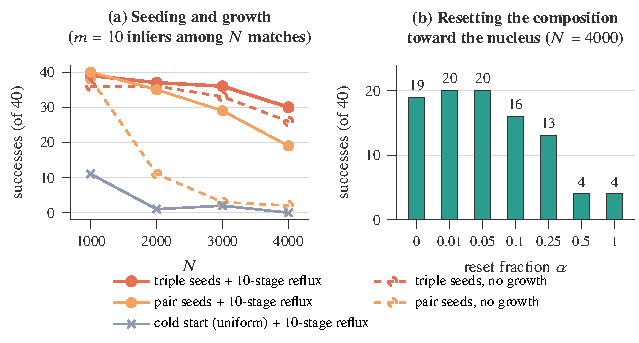
\includegraphics[width=\linewidth]{shared/figures/fig_mechanism.pdf}
\caption{Interventions on the seeding and reflux units (synthetic volume background, $m=10$ generated inliers among $N$ matches, 40 inputs per point; the original estimator configuration with $K=256$ nuclei). (a) Without seeds, growth fails as the feed is diluted; pair seeds without growth fail as well, while purer triple seeds gain less from growth. (b) Resetting a fraction $\alpha$ of each stage's composition to the pair nucleus removes most of the benefit at $\alpha\ge0.5$.}
\label{S-fig:s-mechanism}
\end{figure}

\Cref{S-fig:s-mechanism} removes the seeding and reflux units one at a time on synthetic inputs with ten inliers, using the original estimator configuration ($K=256$ nuclei, the count readout and two hard refits). The inputs use an earlier draw of the Bunny volume generator (master seed 2026102501 and one fixed 4000-vertex source sample). Across the four values of $N$, we retain the same ten inliers, noise, pose and all matches present at smaller $N$. Without seeds, ten stages of growth from a uniform start recover 11/40 inputs at $N=1000$ and 0/40 at $N=4000$. With pair seeds the same growth recovers 40/40 and 19/40, and triple seeds recover 39/40 and 30/40. Without growth, pair-seeded success falls from 38/40 to 2/40 as $N$ grows, while triple seeds start purer and gain less from growth (26/40 to 30/40 at $N=4000$). We test retention by resetting part of each pair-seeded phase toward its initial composition at every stage: the factor $w_i^{(s)}$ of \main{\cref*{eq:growth}} is replaced by $(1-\alpha)w_i^{(s)}+\alpha w_i^{(0)}$. The support factor still uses the current composition. Thus $\alpha=0$ gives the original update, while $\alpha=1$ reapplies the nucleus weights at every stage. Small resets ($\alpha\le0.05$) change little, and $\alpha\ge0.5$ leaves 4/40.

\subsection{Removing units on the frozen benchmark}

The frontend was designed for correspondence sets with very few correct matches. Real benchmarks contain such pairs (\main{\cref*{sec:product}}) but do not allow direct control of the inlier count, which motivates the synthetic tests. We regenerate the benchmark from its fixed seeds and remove one unit at a time (\main{\cref*{fig:sparse}}), and then draw fresh inputs (\cref{S-sec:s-fresh}). The frozen \ngr{} and TurboReg reproduce the recorded counts exactly; the updated C++ MAC differs from the earlier array implementation on one cube input. SC$^2$-PCR, rerun here, registers 57, 95 and 13 of the 250 inputs on the cube, sphere and volume conditions, compared with the recorded counts of 52, 95 and 14. The arms of \main{\cref*{fig:sparse}} are ``no growth'', the same nuclei fitted directly, and ``cold start'', one uniform phase grown for ten stages. Here we also report ``MAC, count readout'': the width-matched C++ MAC candidates selected by the count readout that \ngr{} applies to pair nuclei; on the volume background the native MAC bar retains its own MAE choice, while the count-readout bar is a separate control.

On the cube condition (five inliers among 500 matches) \ngr{} registers 69.2\% of the inputs, against 58.4\% for the width-matched C++ MAC (\cref{S-sec:s-maccpp}) and 58.8\% for TurboReg (paired $+54/-27$ and $+54/-28$, Holm $p<0.01$). On the sphere condition (three inliers among 1000 matches) it registers 64.8\% against 52.4\% for MAC and 26.4\% for TurboReg ($+100/-4$ against TurboReg, Holm $p=10^{-24}$). On the volume condition, it registers 19.2\% against 15.6\% for MAC (not significant) and 9.2\% for TurboReg ($+35/-10$, Holm $p=5\times10^{-4}$). On the cube, fitting the same seeds without growth lowers recall to 55.2\%, below both baselines ($+57/-22$ for growth, Holm $p=3\times10^{-4}$), and a cold start reaches 3.2\%. On the sphere growth adds $+18/-3$ under \ngr{}'s count readout (with the MAE readout both reach 130). The readout accounts for part of this difference: MAC with \ngr{}'s count readout reaches 63.2\%, not significantly below 64.8\%. With triple nuclei (volume background) growth leaves \ngr{}'s output unchanged (48 either way); its pools contain a correct pose slightly less often (170 against 180). These purer seeds leave less scope for enrichment by growth.

\subsection{Fresh draws and thinned real scans}
\label{S-sec:s-fresh}

\begin{figure*}[t]
\centering
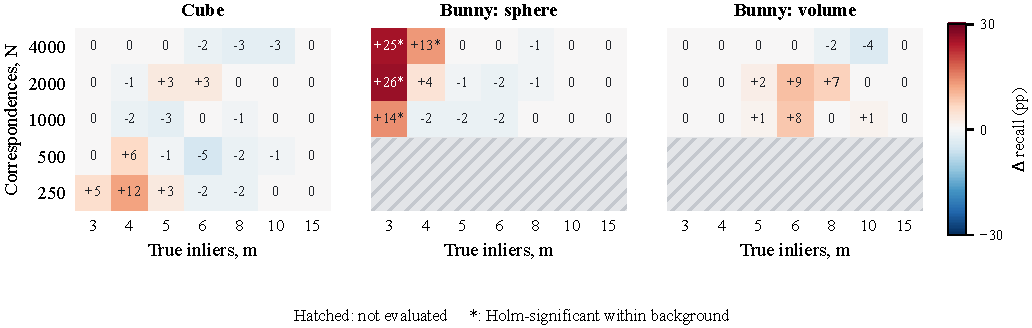
\includegraphics[width=.95\linewidth]{shared/figures/fig_s13.pdf}
\caption{Fresh synthetic inputs (100 per cell): \ngr{} minus the better of six baseline arms (three methods, two parameter sets each), in percentage points; red: \ngr{} higher. Stars: Holm-significant within a background; hatched cells were not evaluated. The sphere cells lose significance once MAC uses \ngr{}'s count readout.}
\label{S-fig:s-fresh}
\end{figure*}

\paragraph{Fresh-draw protocol.} We draw new inputs from the three benchmark generators using master seed 2026110301. \Cref{S-fig:s-fresh} has 77 cells of 100 inputs: $m\in\{3,4,5,6,8,10,15\}$ with $N\in\{250,500,1000,2000,4000\}$ on the cube background (35 cells, independent draws) and $N\in\{1000,2000,4000\}$ on the sphere and volume backgrounds, where inliers are sampled from the first 1000 Bunny vertices. For each of these backgrounds, the 21 cells share poses and source clouds and are nested in $N$ and $m$. Each baseline runs with both of its parameter sets, the original and the calibrated one, and \ngr{} is compared with the better of the six baseline arms in each cell (exact McNemar test, Holm over the cells of a background).

On these 7700 inputs, with each baseline given the better of its two parameter sets, \ngr{} is never significantly worse than the best baseline arm, with the largest gains on the most dilute inputs. With three inliers on the sphere background it registers 67, 48 and 29 of 100 inputs at $N=1000$, 2000 and 4000, against 53, 22 and 4 for the best baseline arm (Holm $p\le0.05$ in each cell). With four inliers at $N=4000$, the counts are 84 against 71. With three inliers, growth adds 5--10 inputs per cell and loses none ($+22/-0$ over the three cells), while summed over all cells its effect is smaller ($+86/-45$ on the cube background, $+19/-11$ on the volume and $+24/-22$ on the sphere; one of the 77 cells is significant after Holm correction). Part of the advantage comes from \ngr{}'s count readout: MAC equipped with it closes the sphere gaps (none of the six cells with three or four inliers is significant). Elsewhere, the frontends perform similarly. The cube advantage of the frozen benchmark does not reproduce with fresh seeds (62 against 63 for MAC with its original parameters).

\paragraph{Thinned real scans.} We also test low inlier counts with the outlier structure of real scans. From the FPFH correspondences of 3DMatch and 3DLoMatch, a pair is eligible if its first 5000 matches contain at least 20 true inliers and 2000 mismatches (residual below $\tau=0.1$\,m under the ground-truth pose; the ground truth is used only to build the input). This criterion admits 1478 of the 1623 3DMatch pairs and 1165 of the 1781 3DLoMatch pairs. The same seeded selection of 200 eligible pairs per benchmark is used in every cell: $m\in\{5,10,20\}$ true inliers and $N-m$ real mismatches with $N\in\{500,1000,2000\}$, nested (the five inliers are among the ten, the mismatches of $N=500$ among those of $N=1000$). Each frontend's native output is scored with the indoor criterion ($15^\circ$, 0.3\,m); finishing is not used. On these 18 cells of 200 pairs (Holm over the nine cells of each benchmark) no frontend is consistently ahead. On 3DMatch SC$^2$-PCR registers more pairs than \ngr{} in 8 of the 9 cells, significantly more than \ls{} with five inliers among 500 matches (84 against 63, $+29/-8$, $p=0.007$), and no difference involving \ngr{} is significant on either benchmark.

\subsection{Decoy clusters}

\begin{figure}[t]
\centering
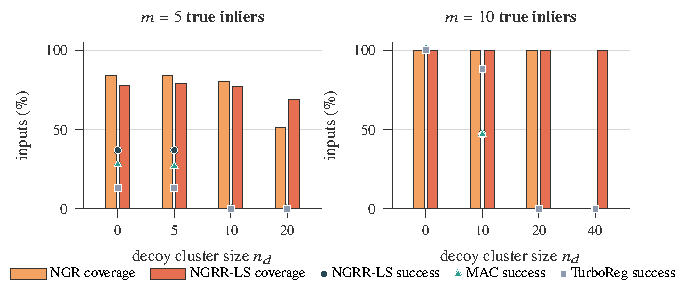
\includegraphics[width=\linewidth]{shared/figures/fig_s14.pdf}
\caption{Decoy clusters (cube, $N=1000$, 100 inputs per bar): $n_d$ outliers are replaced by matches of a second rigid motion. Bars: inputs whose refined candidates contain the true pose. Markers: final success of each frontend's own output (\ngr{} is within one input of \ls{}).}
\label{S-fig:s-decoy}
\end{figure}

Random outliers rarely form compatible clusters. Site capacity gives no significant gain on the cube benchmark above (169 against 173). \Cref{S-fig:s-decoy} plants a decoy on fresh cube inputs with $N=1000$ and $m\in\{5,10\}$: $n_d\in\{0,m,2m,4m\}$ outliers are replaced by matches of a second random rigid motion with the same noise, and the other outliers stay uniform; the baselines use their calibrated parameters. With ten inliers, a 40-match decoy captures every nucleus: the true pose is among \ngr{}'s candidates for 0 of 100 inputs and among \ls{}'s for 100 ($+100/-0$). With five inliers and a 20-match decoy, coverage rises from 51 to 69 ($+22/-4$, Holm $p=0.002$). With smaller decoys, capacity has little effect or slightly reduces coverage (78 against 84 for \ngr{} without a decoy, not significant). Final success is zero for every method once the decoy outnumbers the inliers, because correspondence consensus alone prefers the larger cluster. When the decoy and inlier sets have the same size, performance varies by method: with ten inliers TurboReg registers 88 inputs and \ngr{}, \ls{} and MAC 47 (\ngr{} against TurboReg $+1/-42$, $p=10^{-11}$); with five inliers \ngr{} registers 38, MAC 27 and TurboReg 13.
